%% Submissions for peer-review must enable line-numbering 
%% using the lineno option in the \documentclass command.
%%
%% Camera-ready submissions do not need line numbers, and
%% should have this option removed.
%%
%% Please note that the line numbering option requires
%% version 1.1 or newer of the wlpeerj.cls file, and
%% the corresponding author info requires v1.2

\documentclass[fleqn,10pt,lineno]{wlpeerj}

\title{Elucidating the Role of iRhoms in Breast Cancer Using Meta Co-Expression Analysis}

\author[1]{Abeera Fatima}
\author[1]{Arslan Ali}
\author[2]{Huma Shehwana}
\author[1]{Ayesha Hanif}
\author[3]{Maria Shabbir}
\author[3]{Yasmeen Badshah}
\author[1]{Mehak Rafiq}
\affil[1]{Research Centre for Modelling and Simulation, National University of Sciences and Technology, Pakistan}
\affil[2]{National University of Medical Sciences, Pakistan}
\affil[3]{Atta-ur-Rahman School of Applied Biosciences, National University of Sciences and Technology, Pakistan}
\corrauthor[1]{Mehak Rafiq}{mehak@rcms.nust.edu.pk}

% \keywords{iRhoms, Breast cancer, Meta-analysis, RNA-seq, therapeutic target, WGCNA, Functional enrichment analysis}

\begin{abstract}
Breast cancer is the second most common cancer worldwide as well as in Pakistan. iRhoms are inactive rhomboid proteases play a diverse regulatory role in mammals. iRhoms are remarkable targets to treat ADAM 17 or EFGR-dependent pathological diseases and cancers. This study was designed to provide a clear understanding of the expression and regulation of both iRhom1 and iRhom2 in breast cancer. Meta differential expression analysis revealed that iRhom1 was significantly down regulated, whereas iRhom2 showed heterogenous behaviour in breast cancer patients. Furthermore, a systematic methodology was employed for meta differential expression analysis and meta correlation analysis to find interacting proteins with iRhom1 and iRhom2. Meta transcriptome analysis of RNA-seq datasets showed that iRhoms are not significantly connected to ADAM 17 in breast cancer thus do not support the hypothesis that “iRhoms are upstream regulators of ADAM 17”. iRhom1 is involved in metastasis and angiogenesis incorporation with AXIN which connects iRhom1 with MYC (a gene involved in breast cancer). Study showed significant role of iRhom1 in breast cancer and upregulation of iRhom1 can suppress breast cancer. The possible pathway of iRhom1 in the MAPK, TNF-α and breast cancer pathway in association with AXIN1 and DOCK6, and low expression of iRhom1 can cause neoplasm formation, angiogenesis that ultimately leads to breast cancer. This study enhanced the current understanding about the functional characterization of iRhom1 in breast cancer that will further contribute to its assessment as a potential therapeutic target. However, the specific mechanism needs to be confirmed by subsequent experiments
\end{abstract}

\begin{document}

\flushbottom
\maketitle
\thispagestyle{empty}

\section*{Introduction}

Breast cancer is a complex disease with different biological sub types \citep{Carey2006}. It is the second leading cause of cancer-related to women death and its prevalence rate is increasing day by day \citep{Ludwig2005}. It is a massively complex and diverse disease, though, almost all malignancies shared a set of similar characteristics \citep{Zhang2015}

As, Rhomboids are intra-membrane serine proteases, and they are super family containing many active and inactive proteins. The primary role of these enzymes is the proteolytic cleavage of polypeptide chains of other membrane-anchored proteins \citep{Erez2009, Strisovsky2013}. The critical feature of intra-membrane proteases is that their active site is buried inside the cell membranes \citep{Erez2009}. iRhom is a subclass of rhomboid proteases that has high sequence similarity with rhomboid superfamily. iRhom1/2 are considered inactive rhomboid proteases in humans which do not have the principal catalytic motif present in active rhomboids. It is thought that iRhom1/2 have lost their catalytic function during evolutionary changes\citep{Ha2013}. 

Although they are implicated to have non-protease functions in regulating Epidermal Growth Factor (EGF) and Tumor necrosis factor alpha (TNF-α) signalling pathways\citep{Adrain2012}. This leads iRhoms to have pathological and physiological roles in variety of organism i.e. involved in breast cancer \citep{Idrees2018,Yan2008a}, ovarian cancer \citep{Xu2020}, Tylosis with esophageal cancer \citep{Blaydon2012,Hosur2014}, colorectal cancer \citep{Subramaniam2009}, Alzheimer disease \citep{Lee2016} and many skin diseases \citep{Burzenski2018,Saarinen2012}, etc. Expression of iRhom1 raised in samples of breast cancer and reduced Epidermal Growth Factor Receptor (EGFR) trans-activation could be seen by the silencing of iRhom1 via siRNA \citep{Zou2008}. Therefore iRhoms are remarkable targets to treat  A Disintegrin And Metalloproteinase (ADAM) 17 , also called ADAM17 (tumor necrosis factor-α-converting enzyme) or EFGR-dependent pathological diseases \citep{Li2015}. 


\subsection*{Proposed Work}

In the present study, identification of co-expressed genes was analysed and their possible role in cancer pathways using next-generation sequencing (NGS) data. Differential expression and meta co-expression analysis can be applied to explain this phenomenon and find out real targets. Development of a biological regulatory network to understand the mechanistic of iRhom regulation of ADAM17.

\section*{Methods}

\subsection*{Data Collection}

Publicly available data-sets with GEO accession numbers: GSE110114, GSE69240, and GSE52194 were chosen for breast cancer analysis. Samples from these data-sets were imported to Galaxy \citep{Afgan2018}.

\subsection*{RNA-seq and Differential Gene Expression Analysis}
Raw data files of selected data-sets imported to Galaxy and proceeded for quality control and normalization analysis. FastQC used to check the quality of reads generated, of all data-sets. Trim Galore \citep{Krueger2016} was used to identify portions of adapter sequences present in the read and trim them out.  HISAT2 \citep{Kim2015} used for RNA-seq read alignment to the reference genome. After alignment, count matrix containing the count of each gene was obtained through feature counts tool \citep{Stephani2011}. DESeq2 was used to find differential expression analysis. Selection criteria for deciding Differentially Expressed Genes (DEGs) were based on p-value $\leq$ 0.05.


\subsection*{Co-Expression Analysis Using WGCNA}
\paragraph{Meta-Correlation Analysis}
For meta-correlation analysis, normalised count files were used as input files, this was done separately for iRhom1 and iRhom2. Pearson correlation was calculated for each data-set with iRhom1 and iRhom2, applying the filter of p-value $\leq$ 0.05  to insignificant genes were dropped from further analysis. 

\paragraph{Meta-Correlation Module Detection}
After the calculation of the Pearson correlation for gene pair,  a signed adjacency matrix was established. Subsequently, TOM (topological overlap matrix) was constructed the for which the maximum value is one and the minimum value is zero, using correlation expression values. Then each TOM was used as input for hierarchical clustering analysis, and gene modules were detected by using a dynamic tree-cutting algorithm (deep split $=$ 0-4, minClusterSize $=$ 30, cut height $=$ 0.95).

\paragraph{Identification of Hub Genes}
Meta co-expression gene modules of iRhom1 (identified in the previous step) were next visualized to find hub genes using Cytoscape. For the identification of top ten hub genes degree centrality and MNC (Maximum Neighbourhood Component) method were used using cytoHubba plugin in Cytoscape \citep{Chin2014}. In case of undirected graphs degree centrality measure of a gene/protein/node represents the total number of edges linked to it and MNC declared those genes/nodes as hub genes, which have the maxi-mum number of connections to other genes/proteins/nodes.


\subsection*{Meta Differential Expression Analysis}
Three paired-end data-sets of breast cancer were combined to perform meta-analysis using the normalized count. Initially, each file was normalized separately using DEseq2 tool. The normalized data-sets were then combined to get Meta differential expression analysis using GenemMeta. Forest plots were generated for the expression analysis of iRhom1 and iRhom2 in paired-end data-sets.

\paragraph{Meta transcriptome analysis}
Meta transcriptome was performed in order to check the validity of results produced through meta differential expression and meta co-expression analysis of iRhom1 and iRhom2 containing RNA-seq data-sets. For the transcriptome analysis correlation was calculated with iRhoms.

\subsection*{Functional Enrichment}
For the functional enrichment of DEGs in the selected modules, DEGs in turquoise modules for both iRhom1 and iRhom2 were uploaded to DAVID. Function enrichment of turquoise module containing iRhom1 as performed using DAVID and g:Profiler for result comparison of both tools. To get better results, used g: Profiler results in the form of biological processes (BP), cellular compartments (CC), molecular functions (MF) and KEGG pathways (KEGG). Top ten annotations with –log10 transformed adjusted p-value were used.

\paragraph{Network Enrichment Analysis}
Gene-set enrichment analysis is a useful technique to help functionally characterize large gene lists, such as the results of gene expression experiments. This technique finds functionally coherent gene-sets, such as pathways, that are statistically over-represented in each gene list. 

\section*{Results}
\subsection*{Identification of differentially expressed genes}
The number of genes after applying the normalization process and filtering criteria were reduced to the following for GSE110114, GSE69240, GSE52194 were equal to 13179, 14219 and 12138 respectively. Differential expression analysis of iRhom1 showed significant down-regulation in all three RNA-seq data-sets. Whereas iRhom2 showed inconsistent results as it was significantly up-regulated in GSE110114, significantly down-regulated in GSE69240 and insignificantly down in GSE52194. This shows the variation in the expression levels of iRhom2 in different data-sets as shown in Table \ref{tab:irhom-exp}. 

\begin{table}[h]
\begin{center}
\begin{tabular}{ |c|c|c|c| } 
\hline
Dataset & Gene Name & $Log2(FC)$ & $p-Value$  \\
\hline
\multirow{GSE69240} & iRhom1 & -0.8443 & 0.0005 \\ 
& iRhom2 & -1.4089 & $3.13 e-07$  \\ 
\hline
\multirow{GSE52194} & iRhom1 & -1.443 & $1.2 e-05$ \\ 
& iRhom2 & -0.464 & 0.2653   \\ 
\hline
\multirow{GSE110114} & iRhom1 & -0.6354 & 0.0009  \\ 
& iRhom2 & 1.575 & $3.40 e-14$ \\ 
\hline
\end{tabular}
\caption{\label{tab:irhom-exp}Expression values of iRhom1 and iRhom2 in RNA-seq datasets.}
\end{center}
\end{table}

\subsection*{Meta-differential expression analysis}
Meta differential expression analysis was done to see whether iRhoms expression was consistently perturbed across several studies. To get meta differential expression of all genes, GeneMeta an R package was used.  As it can be seen from Figure \ref{fig:forest-plot}, iRhom1 mean difference (dashed line) lies on the negative side of the null hypothesis hence the difference seen is carried across even when several studies are combined. The grey boxes represent the size effect each study has had on the mean of iRhom1. Whereas, for iRhom2 it can be seen that the null hypothesis is proven to be true, which means that even when pooled together iRhom2 is not differentially expressed in diseased state. 

\begin{figure}[ht]
\centering
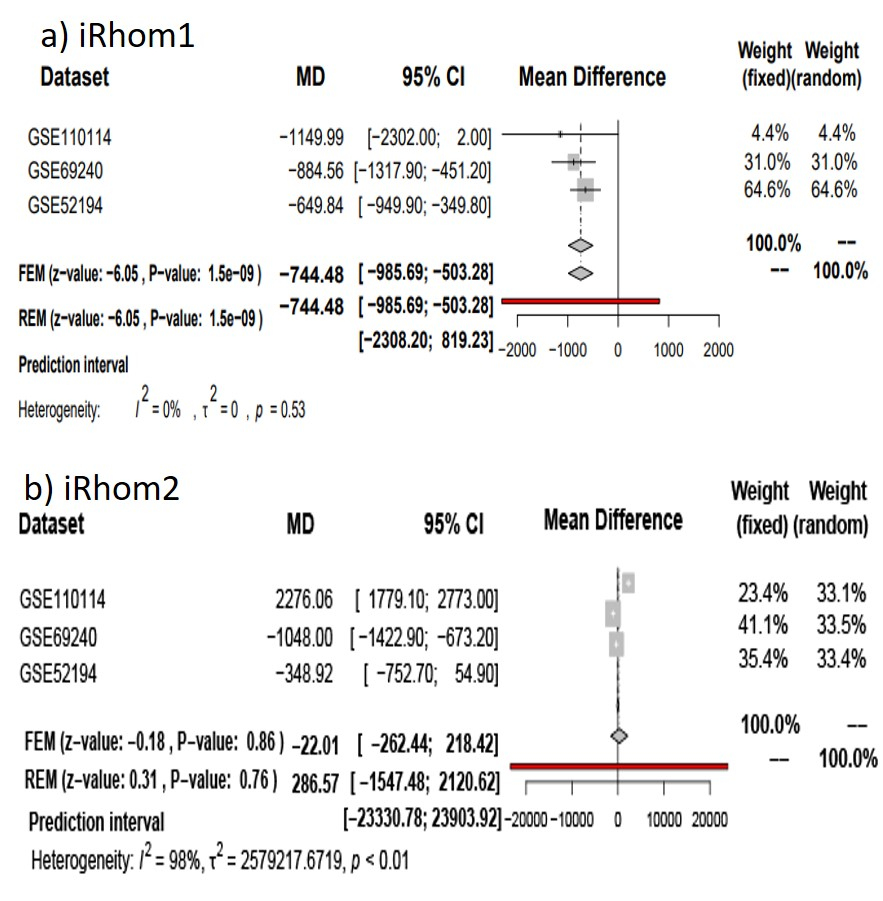
\includegraphics[width=\linewidth]{forest-plot.jpg}
\caption{Meta-analysis of the differential expression of the (a) iRhom1 and (b) iRhom2 genes in breast cancer compared to normal samples. This figure shows a forest plot with filled squares representing the point estimates and error bars indicating the 95\% confidence interval around the standardized mean difference. The summary effect statistics is shown as a grey colour filled diamond whose dashed vertical line (centre) shows the point estimate and the width indicates the 95\% CI (confidence interval).}
\label{fig:forest-plot}
\end{figure}


\subsection*{Meta co-expression analysis using WGCNA}
Meta co-expression network analysis was performed to get genes of interest that are highly correlated with iRhom1 and iRhom2 in breast cancer. Through WGCNA, five gene and eight modules were identified in for iRhom1 and iRhom2 respectively. Dendrograms obtained provided in Figure \ref{fig:gene-dendo}. Each colour represents the clustering pattern of genes into respective modules. The turquoise module (n=903) containing iRhom1 and green module (n=71) containing iRhom2 were identified and selected for further analysis.

\begin{figure}[ht]
\centering
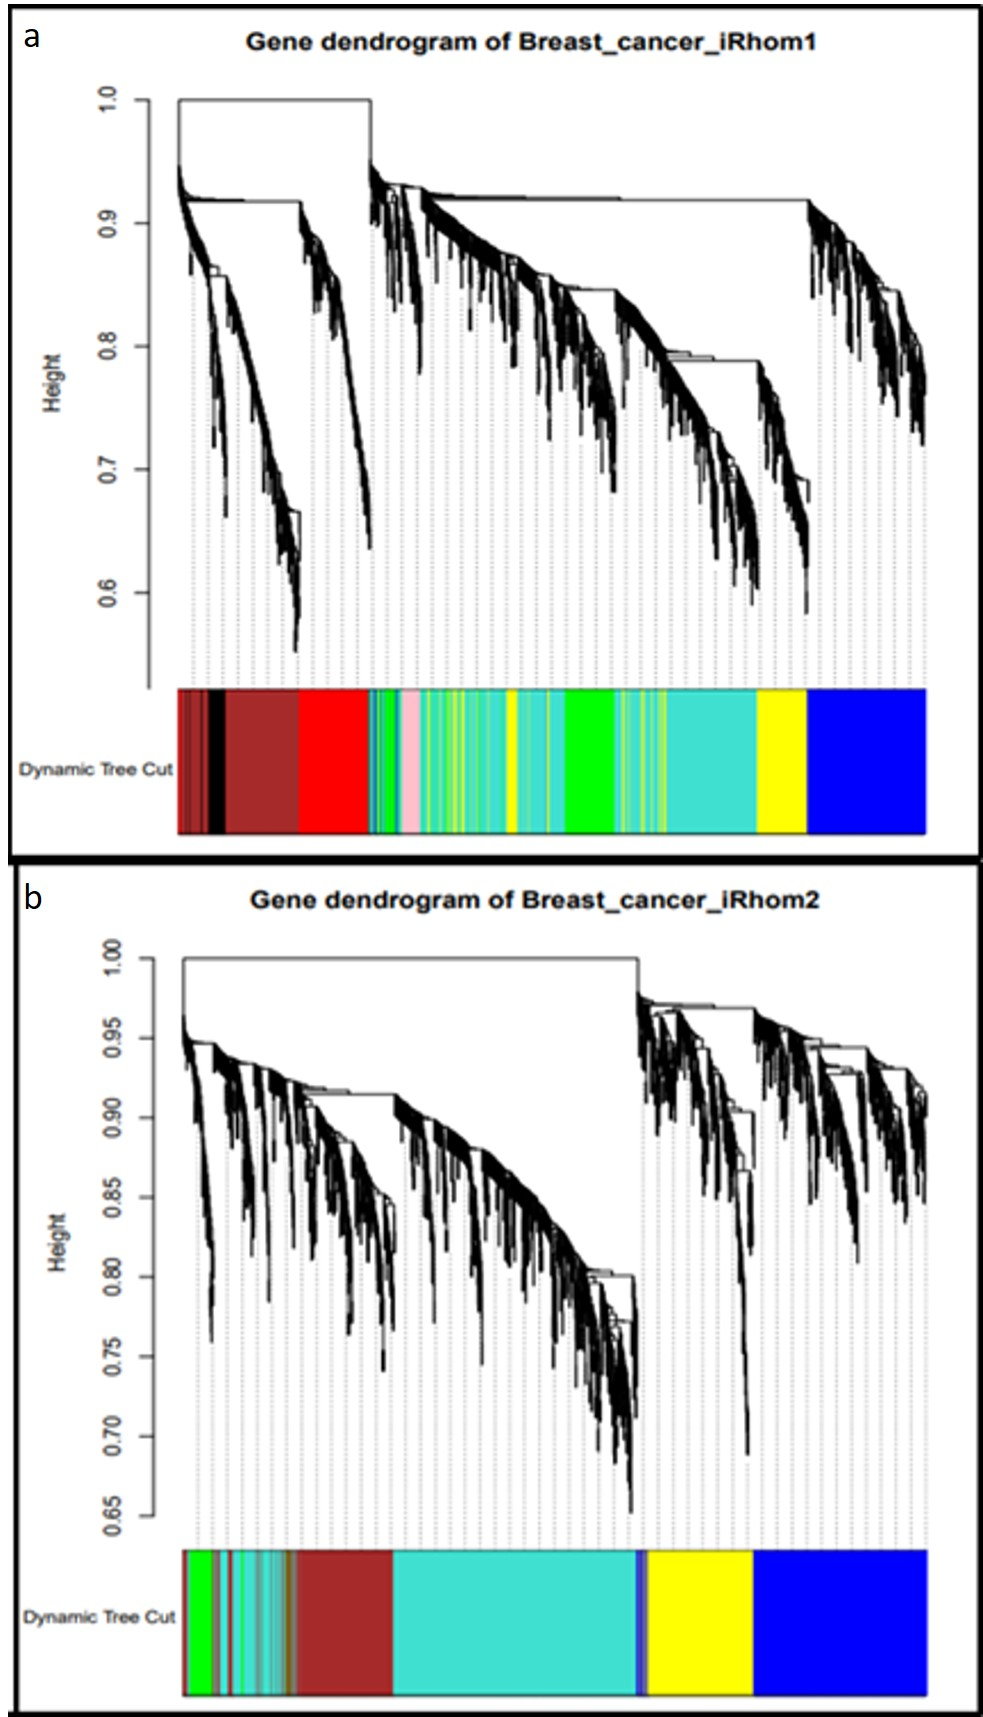
\includegraphics[width=\linewidth]{gene-dendo.jpg}
\caption{Clustering Dendrogram for a) iRhom1 and b) iRhom2 .}
\label{fig:gene-dendo}
\end{figure}

Then the modules were correlated with disease status (external trait) to find their biological significance. A soft threshold of p-value $\leq$ 0.05 was set as criteria to find the significance of correlated modules. In the case of iRhom1 module turquoise showed the highest negative correlation (-0.90) with a good significance level $ 4 e-25$ shown in Figure \ref{fig:mod-trait}. Module turquoise module (containing iRhom1) showed 90 \% correlation with cancer status. This module contains 669 total genes. Whereas in case of iRhom2, green module (containing iRhom2) showed poor correlation (0.063) with insignificant p-value  $\geq$ 0.6. This module contained 71 total genes including iRhom2, showed 6.3 \% correlation with cancer status. Module membership vs diseases state correlation ship were calculated for modules in which iRhom1 and iRhom2 were present.The turquoise module containing iRhom1 the correlation was 0.93 (p-value $\leq$ $1 e -200$ whereas for the green module containing iRhom2 showed poor correlation of 0.22 (p-value $\geq$ 0.065. To study this scatter plots of meta differential expression vs meta correlation were calculated as can be seen in Figure \ref{fig:scatter-plot}. The all genes were plotted with against their differential expression and their correlation with iRhoms. It can be inferred from the figure in the case of iRhom1 the differentially expressed genes show high correlationship with iRhom of interest. Whereas this is not the case with iRhom2 no such pattern can be seen. Hence it can be said that in case of breast cancer genes  that are differently expressed in tumors are correlated with iRhom1, hence it plays an essential role in the breast cancer pathway, though the same can not be said for iRhom2.    
\begin{figure}[ht]
\centering
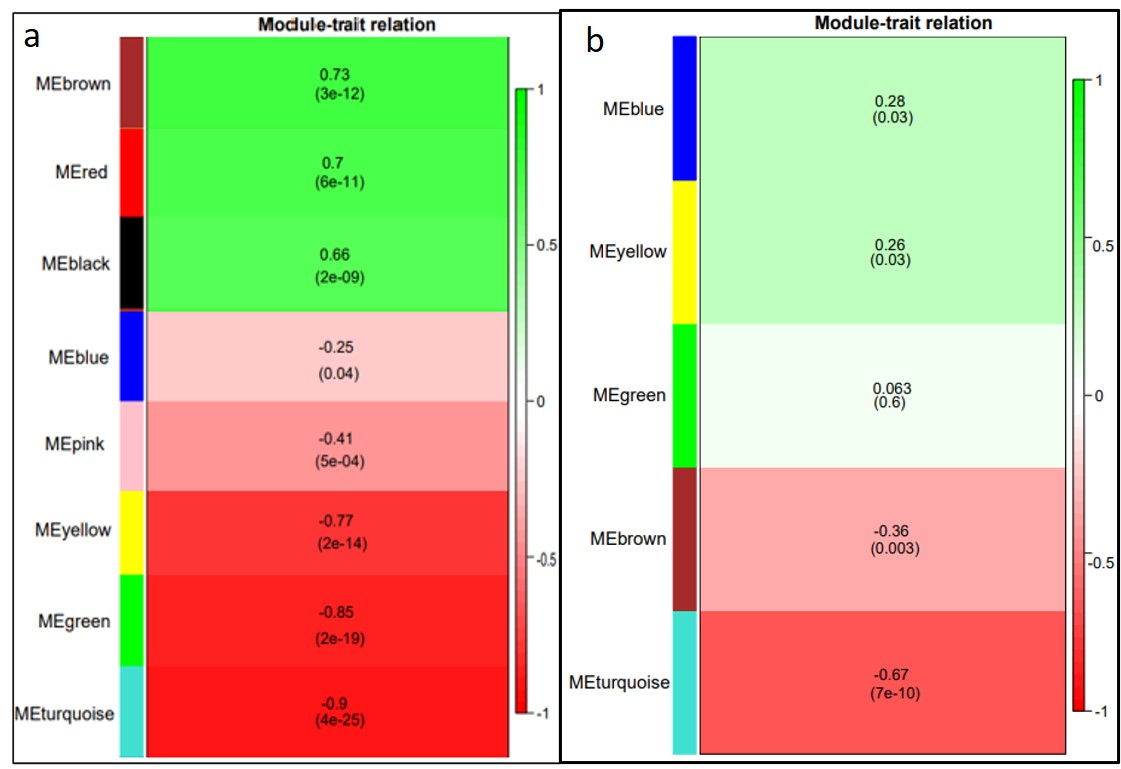
\includegraphics[width=\linewidth]{mod-trait.jpg}
\caption{Heat Maps for (a) iRhom1 and (b) iRHom2}
\label{fig:mod-trait}
\end{figure}

\begin{figure}[ht]
\centering
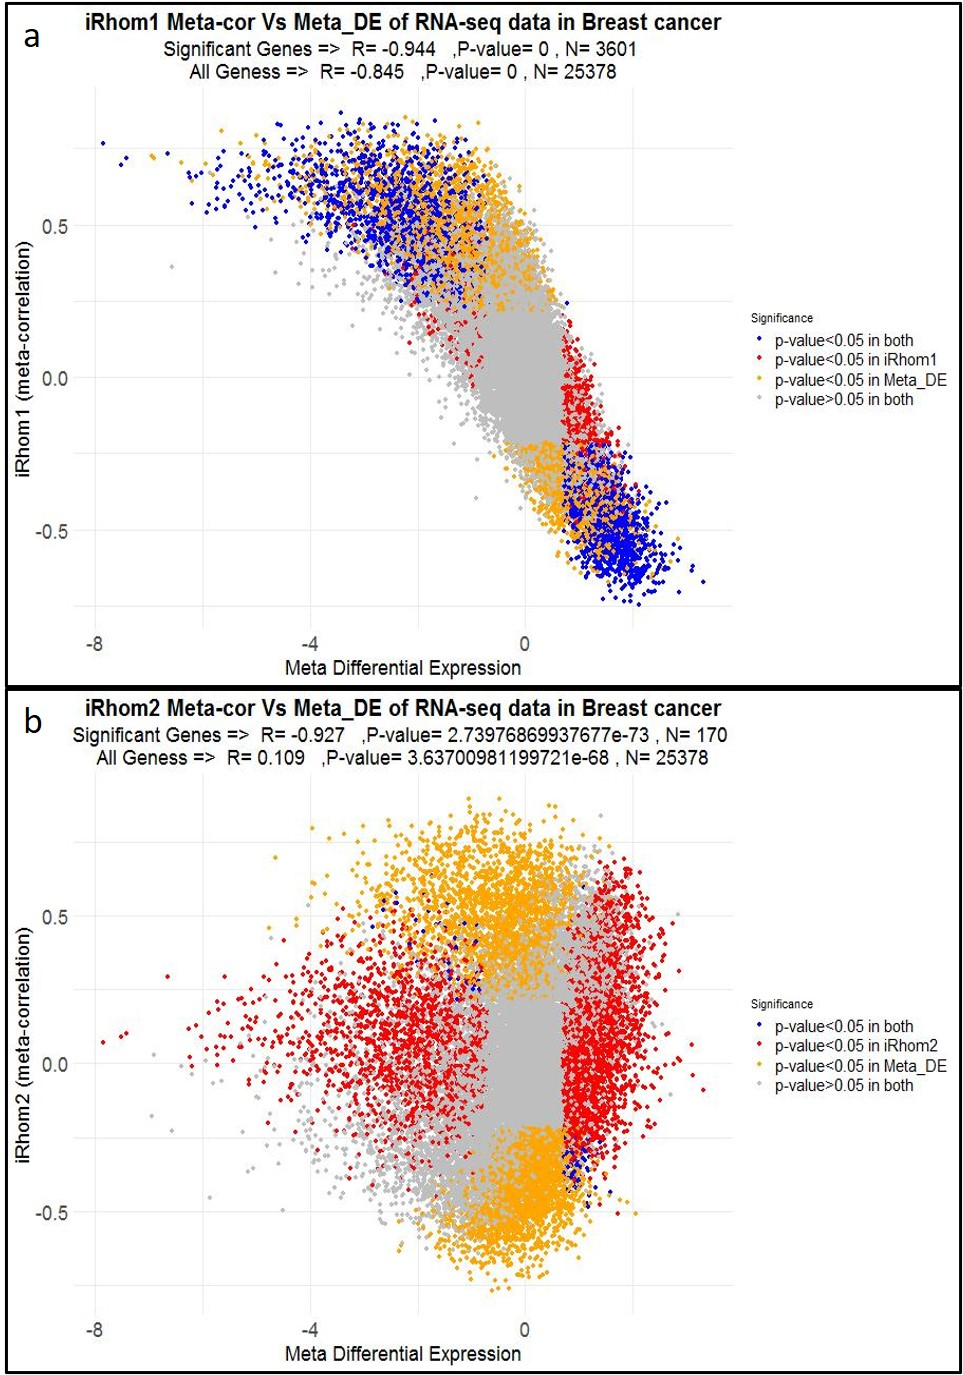
\includegraphics[width=\linewidth]{scatter-plot.jpg}
\caption{Scatter plot analysis of meta differential expression data versus meta correlation of a) iRhom1 and b) iRhom2 in breast cancer}
\label{fig:scatter-plot}
\end{figure}

\subsection*{Identification of Hub Genes}
Since iRhom1 from the previous results showed direct involvement in breast cancer as opposed to iRhom2. Hub genes were identified using Cytoscape plugin cytoHubba using MNC and Degree method.Top ten hub genes are shown in Figure \ref{fig:hub-genes}.  Furthermore Meta differential expression values were used to characterize the model based on differential expression. Even though iRhom1 was not identified in the top 10 hub genes, network analysis of iRhom1 shown in Figure \ref{fig:network-irhom1}
\begin{figure}[ht]
\centering
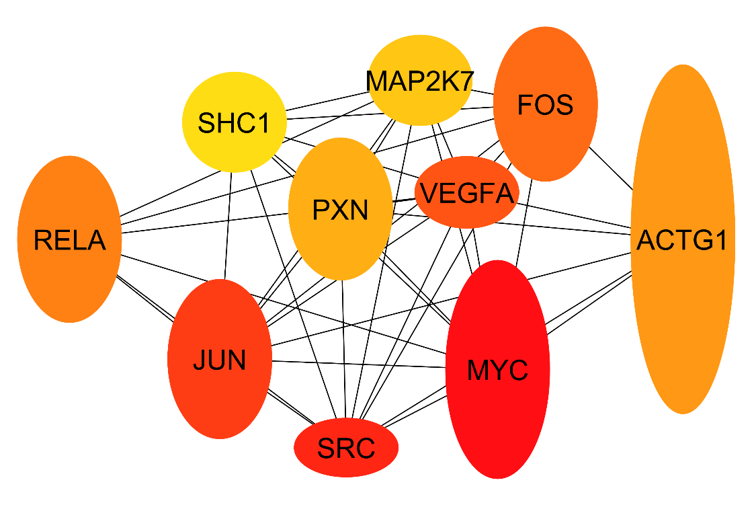
\includegraphics[width=\linewidth]{hub-genes.png}
\caption{Co-expression network of Hub-genes as identified using degreen and mnc}
\label{fig:hub-genes}
\end{figure}

\begin{figure}[ht]
\centering
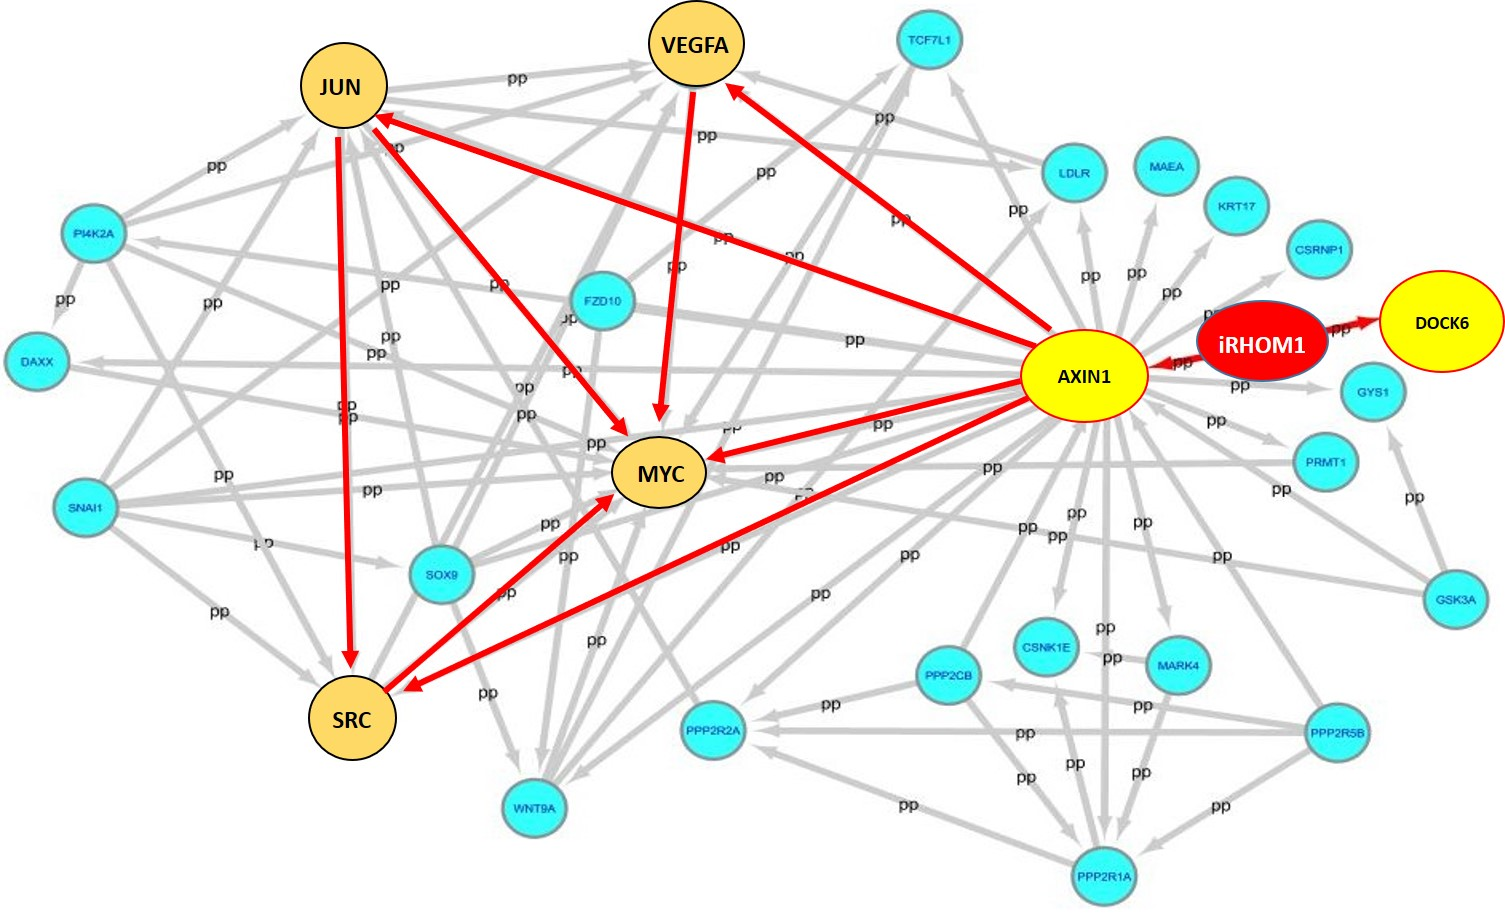
\includegraphics[width=\linewidth]{network.jpg}
\caption{Network analysis of iRhom1 using expression values and string database. iRhom1 is linked to 2 genes Axin1 and Dock6, Axin1 links to three main hub genes as identified }
\label{fig:network-irhom1}
\end{figure}

\subsection*{Link to ADAM17}
Several studies have reported antagonistic role of iRhoms in tumourigenesis and other diseases i.e. either they are involved in negative regulation of EGFR ligands via ERAD pathway or they positively regulate EGFR ligands leading to EGFR signalling pathway. There are parallel studies suggesting iRhom mediated cleavage of EGFR ligands via ADAM17 dependent or ADAM17 independent pathway \citep{Al-Salihi2020}. 
These pseudoproteases are important for the maturation and trafficking of ADAM17 also known as TACE(TNF-$\alpha$ converting enzyme) to plasma membrane from Endoplasmic reticulum through Golgi apparatus and also linked to the fates of TNF-$\alpha$   and EGFR ligands\citep{Lee2016}.It has also been suggested that both of the proteins are up-regulators of ADAM17. A scatter plot to test the correlation between iRhom1 and iRhom2 and iRhom1 and ADAM17 were made. As it is visible in the Figure \ref{fig:adam-link} iRhom1 has no link with ADAM17 or iRhom2 in case of breast cancer. 

\begin{figure}[ht]
\centering
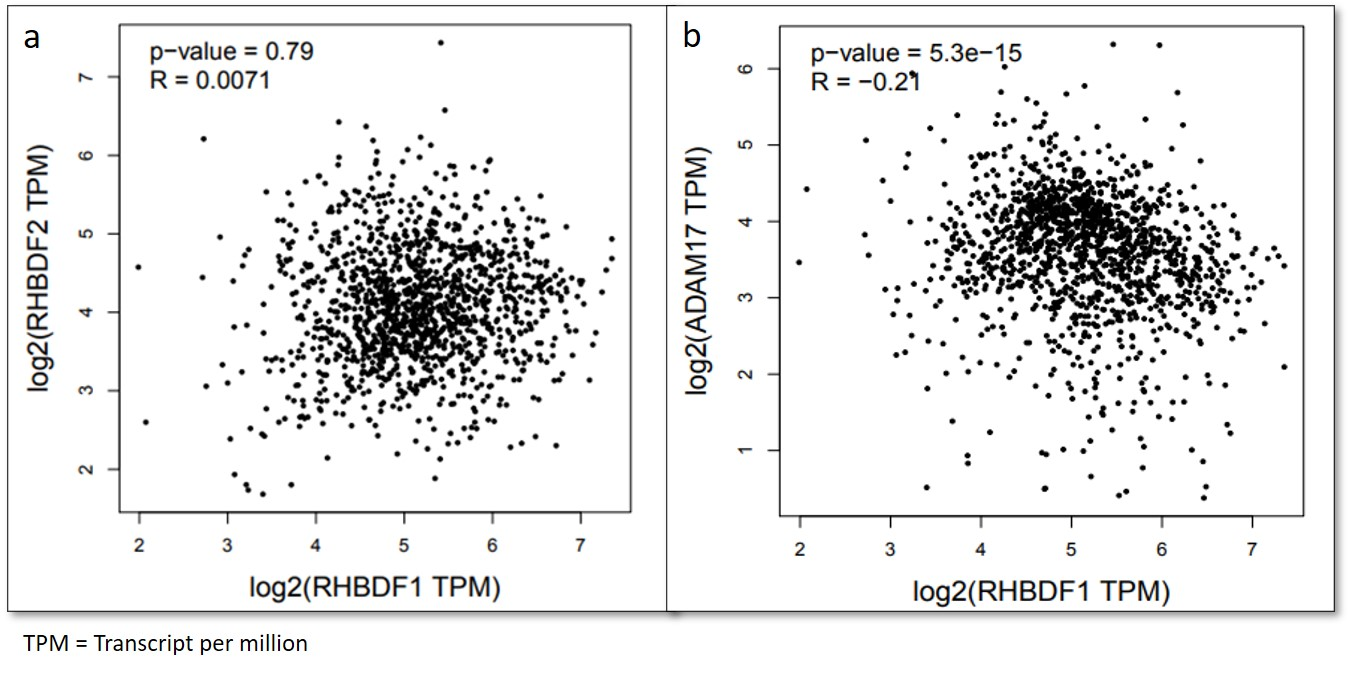
\includegraphics[width=\linewidth]{link.jpg}
\caption{Scatter plots of (a)iRhom1 (RHBDF1) vs iRhom2 (RHBDF2) (b) iRhom1 (RHBDF1) vs ADAM17  Transcript per million for all three data-sets meta-differential expression analysis }
\label{fig:adam-link}
\end{figure}

\section*{Discussion}
In mammalian cells, growth, proliferation and differentiation is held by EGFR signaling pathways. Important EGFR ligands such as AREG, HB-EGF and EGF binds to EGF receptors(EGFR’s) as proproteins and must be cleaved to shed into the extracellular compartment in active form for signaling. But these ligands are membrane tethered and  different proteases like active rhomboids and pseudoproteases via client proteins helps in cleaving membrane bound EGFR proligands to convert them into biologically active proteins during proliferation (Dulloo, Muliyil & Freeman, 2019). Moreover, the physiological targets as substrate for enzymes like iRhoms are critical to find but many studies on mice models and D. melanogaster suggest EGF ligands as potential substrates for these pseudo enzymes(Urban & Dickey, 2011).
ADAM17 is synthesized in endoplasmic reticulum as an immature form containing an inhibitory prodomain that prevents its proteolytic activity. iRhom forms a complex with FRMD8 protein which is an interacting protein . This complex along with an enzyme called furin helps in the removal of the prodomain and converts the ADAM17 into active form in golgi(Adrain & Freeman, 2012). The mature ADAM17 trafficks to the plasma membrane with iRhom. The binding of 14-3-3 proteins to iRhom N-terminal domain seems to result in weakening of interaction with ADAM17 at the cell surface. The ADAM17 at the plasma membrane then simultaneously cleaves the EGFR ligands and TNF-a ligands via its sheddase activity thereby mitigating the onset of signaling and inflammatory pathways (Dulloo, Muliyil & Freeman, 2019).Without iRhoms there is no ADAM17 maturation and therefore no ADAM17 activity. Mounting literature and evidence from physiological and molecular data claims the alterations in ADAM17 function due to evident mutations or deletions in N terminal (Blaydon et al., 2012) (Brooke et al., 2014)  (Siggs et al., 2014) (Li et al., 2015).
Whereas, (Hosur et al., 2014) debate on EGFR signaling independent of ADAM17 and states that cleavage of EGFR ligands occurs via essential residues within peptidase domains. The study was challenged  few months later by (Siggs et al., 2014) on the idea of ADAM17 independent mediated regulation of EGFR ligand. Later in 2018, conditional deletion of ADAM17 , in RHBDF2   impaired AREG mediated sebaceous gland enlargement , wound healing and alopecia suggesting ADAM17 is essential for shedding of EGFR ligand (Hosur et al., 2018).  Another study on breast cancer has stated iRhoms can regulate proliferation during tumorigenesis via GPCR (G-protein coupled receptor) signaling by transactivation of EGFR signaling (Christova et al., 2013). EGFR transactivation via IRhom-1 in Breast Cancer promotes the survival of epithelail tumor(Miyazaki et al., 1998).
Parallelly, some studies claim iRhom to be negative regulators of EGFR ligands (Adrain & Cavadas, 2020). Evidence showed onset of sleep like phenotype in D.melanogaster is because of iRhoms are involved in negative regulation of EGFR signaling through ERAD pathway in nervous system whereas active rhomboids regulate cleavage of EGFR membrane bound precursors [16] .There exist some conserved mechanistic link between mammals and drosophila in regulation of EGFR signaling and in maintaining cell quality control machinery for efficient trafficking (Etheridge et al., 2013). iRhoms can negatively regulate EGFR signaling via breakdown of EGF like substrates(Lee, Nam & Choi, 2016).They increase ERAD activity by bringing clients passively by delaying ER retention, hence enhancing the chance of exposure to ERAD machinery. While (Zettl et al., 2011) suggest that they can perform this mechanism by specifically destabilizing some substrates in ER, inhibiting their access to active rhomboids leading to degradation. Apart from cancer, (Lyu et al., 2018) identified the high expression of iRhom2 in renal tubules as target of PPARG thus promoting EGF degradation via ERAD.
This paradoxical behavior of iRhoms was tested using meta co-expression analysis on RNA-seq datasets of breast cancer patients, in order to get highly co-expressed genes with iRhom1 and iRhom2 among all breast cancer datasets.


The focus of the study was to understand the role of iRhoms in breast cancers. It is the 2$^{nd}$ most prevalent cancer in Pakistan and worldwide (Khan, 2009),(Siegel, Miller & Jemal, 2019). Leading to many untimely deaths each year (Jemal et al., 2010), (Siegel, Naishadham & Jemal, 2012). As mentioned earlier iRhoms are inactive rhomboid proteases, present in nearly all  prokaryotes and eukaryotes. Previous studies had have suggested that iRhoms are up-regulated in breast cancer using various knockdown studies, mostly done in mice (Yan et al., 2008b),(Hosur et al., 2014). Furthermore these studies suggested that the iRhoms were the upstream regulators of TNF-α converting enzyme (ADAM17) which is involved in the cleavage of TNF-α and EGFR ligands at the cell membrane (McIlwain et al., 2012),(Maney et al., 2015), (Künzel et al., 2018). This cleavage leads to hyper-activation of the PI3K/AKT pathway TNF-α pathway causing abnormal growth of cells, causing cancer. At initial stages implication of iRhom1 was reported in breast cancer with higher levels compared to normal breast tissues, and silencing of the iR-hom1 gene resulted in apoptosis in breast cancer cell lines(Tang et al., 2009).  Neverthe-less the exact pathway is still unknown (Düsterhöft et al., 2019). This hypothesis was tested using meta co-expression analysis on RNA-seq datasets of breast cancer patients, in order to get highly co-expressed genes with iRhom1 and iRhom2 among all breast cancer datasets. Meta-expression divides all the differentially expressed genes into dif-ferent modules based on their correlation to the disease. The turquoise module (n=669) containing iRhom1 showed a very strong negative correlation (-0.9) with disease status while that of iRhom2 green module (n=71) sowed poor correlation (0.06) with breast cancer status. Based on poor correlation with insignificant p-value to disease of iRhom2, it was not considered for further analysis. However, module containing iRhom1 showed promising results by showing a strong correlation with disease status as well as a strong correlation high with significance in module membership versus gene significance. It showed that all genes present in the iRhom1 module are highly implicated in breast cancer as well as their correlation with the iRhom1 gene in disease. Initially, it was thought that iRhom1 and iRhom2 function complementary to each other due to se-quence similarity (Dulloo, Muliyil & Freeman, 2019). Based on this discovery, it was assumed that iRhom1 has the same possible role. Yet there was no clear evidence for their exact function and mechanism. This was refuted by the present work, as iRhom2 had no co-relation with breast cancer. This suggest the possibly different regulation of both. GEPIA results shows that iRhom1 and iRhom2 have negligible or no correlation with each other. Therefore, it is clear now that both iRhom1 and iRhom2 have different regulatory functions and they do not work complementary to each other in case of breast cancer.  GEPIA2 also support this study that iRhom1 has negligible correlation with ADAM17 which means iRhom1 is not involved in the maturation and trafficking of ADAM 17 in case of breast cancer. Two directly connected genes of iRhom1 (RHBDF1) in the Meta co-expression network are AXIN1 and DOCK6. These genes show the most similar gene expression pattern with iRhom1. Both the MNC and degree methods gen-erated the same top ten hub genes, which increases the importance of identified hub genes. The degree method was used for further analysis. RELA and MYC were the high-est connected genes in the entire meta co-expression network. 

MYC is one of the important gene for the cell growth, proliferation, differentiation, metabolic and apoptotic activities(Kortlever et al., 2017). Deregulated expression of MYC leads to the development and progression of breast cancer (Vita & Henriksson, 2006). Transcriptional regulation is one of the reasons for deregulation of MYC in breast cancer and has a strong correlation with loss of tumor suppressor and activate cancer pathways. Although MYC show heterogenous behaviour in case of breast cancer (Glöckner et al., 2002),(Heselmeyer-Haddad et al., 2012). The component tumor cells of many human breast cancers show persistent heterogeneity can be seen in the expression of Myc in the component tumor cells of many samples of breast cancer in human (Parajuli et al., 2017). Study showed that individually, ubiquitously Mychigh or Myclow mammary tumor cells show distinctly diverse features, each of which significantly con-fines carcinogenic potential. Specifically, it suggested that therapeutic efficacy depends on disrupting the balance between proapoptotic and antiapoptotic signals: MEK inhibi-tion blocks antiapoptotic signaling, and so predominantly affects the Mychigh clone, whereas COX2 inhibition increases proapoptotic signalling, thereby reinforcing the im-pact of MEK inhibition on the Myclow cells (Kreuzaler et al., 2019). AXIN1 gene en-codes cytoplasmic protein which is involved in the regulation of G-protein signalling domain and a dishevelled and axin domain. Reduced potential of AXIN1 has been re-ported in esophageal squamous cell carcinoma having correlation with tumor progres-sion. Chimge et al. reported AXIN1 as potential target for ER+ breast carcinoma. More-over, RELA and DOC6 also have critical role in breast cancer and all these genes are as-sociated with iRhom1 in this study. So, in the future there is a need to understand the exact mechanism and pathway between these proteins. Which may play an important role in the therapy of breast cancer.  ADAM 17 regulation is a very complex process, which is not fully understood yet.  In mammals (first time in mice), function of iRhoms was described as the upstream regulator of ADAM 17 or ADAM 17 to bind with and transport it to Golgi from ER, where furin converts ADAM 17 from immature to mature form and transfer it to cell surface for the cleavage of membrane-bound proteins i.e. TNF-α. Whereas iRhom deficient mice were unable to do so (Lee, Nam and Choi, 2016). Based on this study it was thought that iRhoms are upstream regulators of ADAM 17. Although clear picture of ADAM 17 regulation is still not clear. To date various sub-strates of ADAM 17 are known including TGF-α, TNF-α and amphiregulin etc. but this does not exclude the possibility that these substrate molecules cannot be cleaved with-out ADAM 17 dependent pathway(Burzenski et al., 2018). In the present work iRhom1 has link with TNF-α pathway through the hub genes but no link with ADAM 17. TNF-α linked through hub genes and KEGG pathways with p-values (adj p-value=0.00156266) as shown in Figure 3 14. In the light of above facts and figures iRhom1 has no direct relation with ADAM 17 in breast cancer, and there may be various reasons for this re-ported behaviour which shows to be different from what has been reported earlier. 
\begin{itemize}[noitemsep] 
\item All the previous studies were knockout studies in mice
\item Many similar pathways have different mechanism in mice than humans, which might not translate back to humans
\end{itemize}
In mammals, expression of iRhom2 is limited to few body parts i.e. macrophages whereas iRhom1 expression is found in almost all body parts.


\section*{Conclusions}

Therefore, in the light of all the above-mentioned results, overall expression of iRhom1 is lower in breast cancer, and the meta-analysis does not support the previous studies that declared the iRhom1 also the upstream regulator of TCAE/ADAM 17. Our study suggests that there are some other targets by which iRhom1 interact and involved in cy-tokines release i.e. TNF-α and EGFR ligands. Two direct interactors of iRhom1 were discovered as AXIN1 and DOCK6. Whereas iRhom1 also has a strong correlation with MYC and RELA genes. It is also evident from this study that iRhom2 does not have a role in breast cancer


\section*{Acknowledgments}

I would like to thank my research fellows Ayesha Hanif and Arslan ALi for their help in R programming

\bibliography{abeera.bib}

\end{document}